\documentclass{IEEEtran}
\usepackage[utf8]{inputenc}
\usepackage{graphicx}
\usepackage[ruled,vlined]{algorithm2e} % package for pseudocode

\title{
    \centering
    Distributed Crowd Flow Analysis Using Passive Packet Sniffing\\
    \vspace{10px}
    \small Internet of things Seminar IN4398
}

\author{
    \begin{tabular}{ccc}
        \begin{tabular}{c}
        Jetse Brouwer\\
        {\small 4615964}
        \end{tabular}&
        \begin{tabular}{c}
        David Enthoven\\
        {\small 4502124}
        \end{tabular}&
        \begin{tabular}{c}
        Niels Hokke\\
        {\small 4610148}
        \end{tabular}\\
    \end{tabular}\\
}

\date{\today}

%------------Document----------
\begin{document}
\maketitle

\begin{abstract}
This paper proposes a distributed sensor network for analyzing crowd flow. This enables municipalities, urban developers, city planners and event organizers to study, analyze and optimize crowd flow. The tracking of the crowd will be done by multiple sensor-nodes strategically placed at crowd flow bottlenecks. To measure crowd flow, Wi-Fi activity of smart phones, tablets and other hand-held devices is monitored. Detecting the same devices at different locations over time provides a estimation of the movement of a single device. By using the distributed algorithm developed by the authors and the data gathered by the sensors an insight into the traffic flow on a three-way junction was given.
\end{abstract}

\section{Introduction}
Even when not connected, smart phones and other hand held devices still transmit Wi-Fi messages to search for nearby access points. The number of such packets transmitted may be up to 2000 per hour for an active phone \cite{c1}. Devices to which these messages are not addressed will simply ignore them under normal circumstances. It is possible however to capture and log these messages even if your device is not the desired destination device.

By changing the settings of a device, one is able to perform this so-call sniffing, and record all Wi-Fi transmitted messages surrounding the device. Since these messages includes information about the sender in the form of a MAC address it can be used to uniquely identify the device.

In this paper a distributed network of strategically placed sniffing devices is proposed which will exchange data about devices that pass by the nodes. This makes it possible to track the movements on a per device basis. This is illustrated in Figure \ref{fig:walkingman}.

\section{High level overview}
The proposed network of sniffing nodes will use a low-cost Wi-Fi chip capable of sniffing for packets and means of communicating with other nodes. It will use the MAC address to uniquely identify separate devices. When deploying several of these spread out across roads and near traffic junctions, hand-held devices will move in and out of range of these sensor. Using this data the algorithm analyzes the flows of crowds.

To ensure privacy, the nodes can communicate using a symmetric encryption scheme, as these can be implemented very efficient on lower power devices. A node then only discloses its key to it's direct neighbors, and uses the secure channel to privately transmit the detected mac addresses. For reporting the measurements it only transmits the amount of devices tracked per given direction, and no uniquely identifiable data. 

\begin{figure}
    \centering
    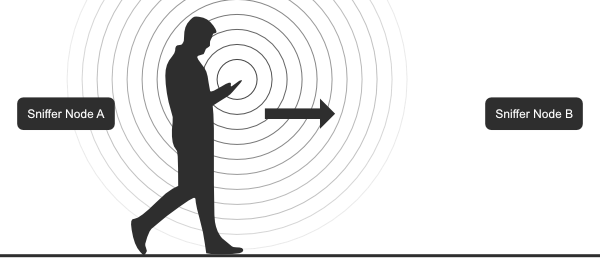
\includegraphics[width=80mm]{images/walkingman.png}
    \caption{The movement of a device between sniffing nodes}
    \label{fig:walkingman}
\end{figure}

\section{Algorithm}\label{sec:algorithm}
The algorithm that was developed for this project supports both direct and indirect detection. This results in the ability of detecting a device's movement, even when an intermediate node fails to detect the device. The algorithm is designed in such a manner that it only needs to communicate with its one-hop neighbor, as the nodes are placed in geometrical graph  the average degree does not significantly increase for a growing network.

\subsection{Direct Detection}
On detection of a packet the node has to figure out if and where the sender has been seen before. To do this every node keeps a list of sightings of it's one-hop neighbors, if the sender of the packet is found there, it knows it the device came from that position. After performing these checks it broadcasts the detected mac address and timestamp to its one-hop neighbors.

In order to ignore devices that move from one node to another through a detour (while not being detected by a in between node) a maximum travel time between nodes is defined. This means nodes can delete sightings from neighbors older than the maximum travel time, which has as a side effect reduced look-up time and memory consumption.

\subsection{Indirect detection}
As devices aren't continuously transmitting and nodes can't sense on multiple channels simultaneous, there is a possibility that a device passes by a node undetected. To combat this we've implemented the notion of indirect detection. Take the example in figure \ref{fig:indirect} where node 1 and node 3 detect the device, but node 2 doesn't. Since node 3 isn't a one-hop neighbor of node 1 it doesn't know about the earlier sighting. however, since node 2 can see the broadcast of the two neighbors it can deduce that it must have traveled passed him without him noticing it. It should only do so if the node self didn't detect him passing and there is no direct path between node 1 and node 3 (to prevent double detection). %and if there are no parallel nodes with onehop to 1 and 3 ?

\begin{figure}
    \centering
    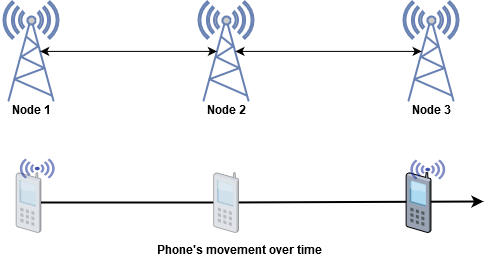
\includegraphics[width=80mm]{images/indirectdetection.png}
    \caption{Example of a hidden detection where the phone moves from node 1 to node 3 past node 2, but node 2 does not receive a packet.}
    \label{fig:indirect}
\end{figure}


\begin{algorithm}
 \If{not seen in the last 30 seconds}{
     \ForEach{neighbor's detection list}{
     remove entries older then max buffer time;
     
     \If{mac address in detection list}{
        remove from detection list;
        
        store route (neighbor ID, own Id, list time, timestamp);
        }
     }
     broadcast (Mac address, timestamp);
 }
 \caption{onPacket(SenderID, Mac address, timestamp)}
\end{algorithm}


\begin{algorithm}

\ForEach{neighbor's detection list}{
     remove entries older then max buffer time;
     
     \If{mac address in detection list}{
        remove from detection list;
        
        \If{no link between SenderID and neighbor and not directly detected}{
            store indirect route (neighborID, SenderID, list time, timestamp);
        }
    }
 }
add to SenderID's detectionlist;
 \caption{onBroadcast(SenderID, Mac address, timestamp)}
\end{algorithm}

\section{Experiments}
To validate the idea, a proof of concept experiment was done. The algorithms described in section \ref{sec:algorithm} were implemented on three Raspberry Pis, as seen in figure \ref{fig:pi}. Using powerbank's the three Pis were able to run in remote locations. For the location a three-way junction in the center of Delft was chosen, see figure \ref{fig:markt}. This location was chosen because it forms a three-way junction without to many allays leaving the junction. An other reason was because at this location a market is held which guarantees a reasonable flow of people.

\begin{figure}
    \centering
    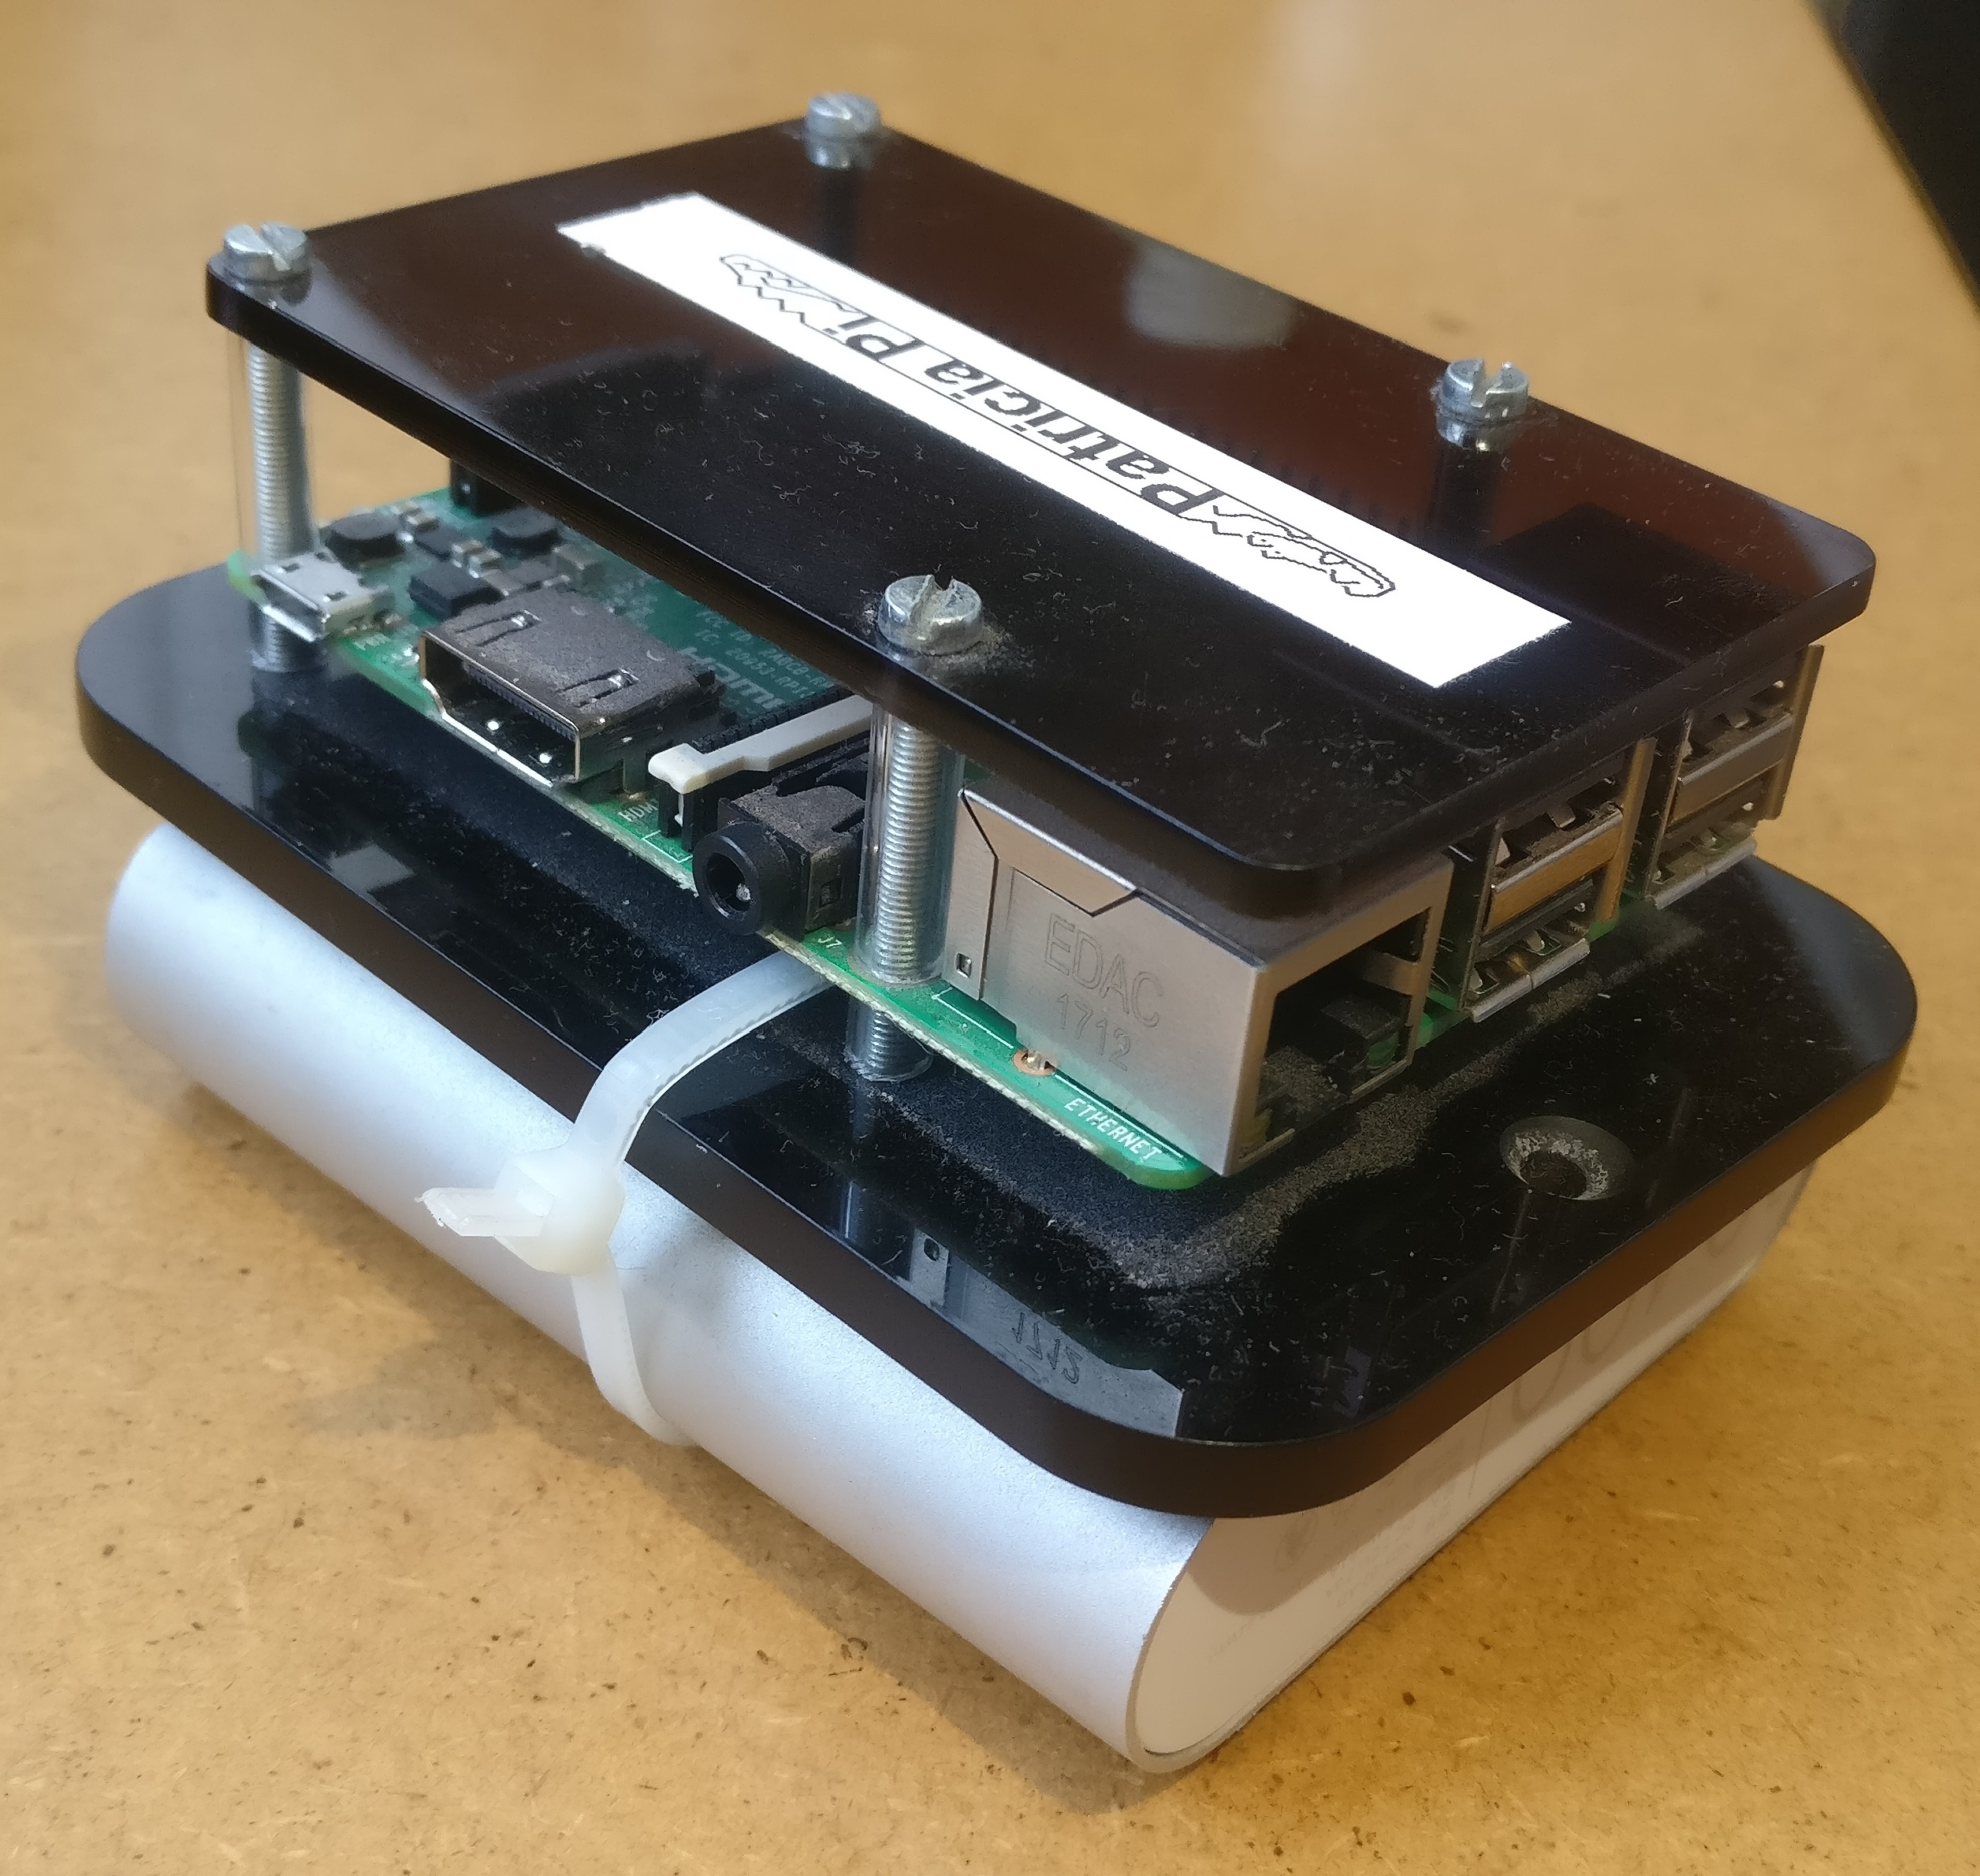
\includegraphics[width=80mm]{images/Pi.jpg}
    \caption{One of the three measuring nodes, existing of a Raspberry Pi 3b and a powerbank.}
    \label{fig:pi}
\end{figure}

\begin{figure}
    \centering
    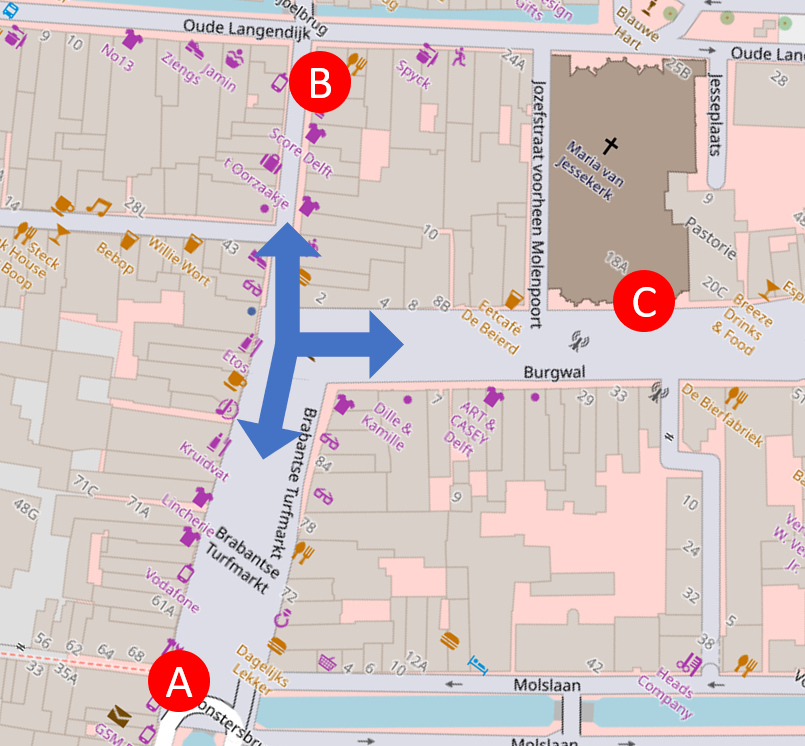
\includegraphics[width=80mm]{images/marketcapture.png}
    \caption{The deployment of the nodes for the experiment. The blue arrows indicates the three way junction being monitored and the red dots the locations of the nodes.}
    \label{fig:markt}
\end{figure}

To increase reproducibility the raw data was recorded instead of being directly processed on the Raspberry Pis. later the recorded data is played back to the Pi's to emulate the actual packet detection. This enables fast development and testing as the algorithm can be tested on hours of data in a matter of seconds.

To validate our results, a short video of 30 seconds at the location of the nodes was recorded every 5 minutes. Using this footage the actual flow was estimated by manually counting people passing by. The assumption is made that the arrival-rate of the people within the five minutes can be approached by a poison distribution. Therefore, the thirty second footage is used to estimate the amount of passers-by for the whole five minute segment by extrapolating.

\section{Results}
The results of the experiment can be seen in table \ref{tab:groundtruth}. The direction column indicates whether the measured flow goes into the intersection or out of the intersection. In this table the in/out-flow estimated by the 30 second video is compared to the detected flow by the system. Taking the inaccuracy of the estimated flow in mind the detected flows approaches the estimated ones. The largest error is in node A, this large error might be due to node A being located in front of a phone shop with more than 40 active phones. These phones may have caused significantly more package collisions or an increase back-off time, causing node A to miss more of the actual flow.

Another proposition of the system is that it can determine the ratio between flows from A-to-B and flows from A-to-C. However, from the ground truth data it is not possible to determine these ratios. This because only the number of people going in/out the junction were counted, and not which branch of the three-way junction was taken.

If all the sniffed flows from table \ref{tab:sniffedtotalroutes} are combined to get the detected flows per node direction in table \ref{tab:groundtruth}, and these flows are divide according to the measured ratios from tables \ref{tab:sniffedinflowratios} and \ref{tab:sniffedoutflowratios}, the exit rate for every node's in/outflow can be estimated.
For example, the total outflow of C, is the inflow of A multiplied by the ratio A-to-C plus the total inflow of B multiplied by the ratio B-to-C.
$$ C_{out} = A_{in} \times Ratio_{A\rightarrow C} +B_{in} \times Ratio_{B\rightarrow C} $$
The results of these value for all three nodes can be found in tables  \ref{tab:inflowresult} and \ref{tab:outflowresult}.
When compared to the actual flows all calculated flows are within 17\%. Except for node A who is 30\% off, which is speculated to be influenced heavily by being in front of a phone store. 

\begin{figure}
    \centering
    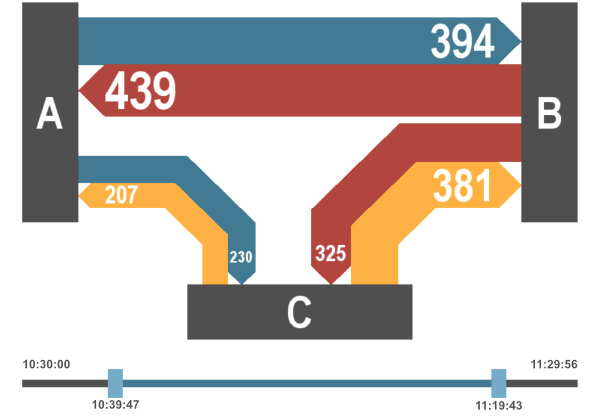
\includegraphics[width=80mm]{images/sankey_tool2.png}
    \caption{Bidirectional sankey diagram to visualize the crowd flow in a set time window}
    \label{fig:sankey}
\end{figure}

\subsection{Data visualization}
To provide an intuitive visualization of the crowd flow a tool was developed which illustrates the flow in the form of a bidirectional Sankey-like diagram. A screen shot of this tool is shown in Fig. \ref{fig:sankey}. The range slider in the bottom of the interface provides a quick way to look at a specific time window.

\begin{table}
    \begin{minipage}{.5\linewidth}
        \centering
        \caption{Estimated ground truth from videos and detected}
        \label{tab:groundtruth}
        \begin{tabular}{|l|l|l|l|}
        \hline
        Node & Direction & Video    & Detected \\ \hline
        A    & In        & 973      & 730      \\ \cline{2-4} 
             & Out       & 1018     & 749      \\ \hline
        B    & In        & 995      & 928      \\ \cline{2-4} 
             & Out       & 810      & 905      \\ \hline
        C    & In        & 640      & 672      \\ \cline{2-4} 
             & Out       & 680      & 676      \\ \hline
        \end{tabular}
        
    \end{minipage}%
    \begin{minipage}{.5\linewidth}
    
        \centering   
        \caption{Detected Total Per Routes}
        \label{tab:sniffedtotalroutes}
        \vspace{10px}
        \begin{tabular}{|c|l|}
        \hline
        Flow               & Detected \\ \hline
        A $\rightarrow$ C  & 267       \\ \hline
        B $\rightarrow$ C  & 409       \\ \hline
        B $\rightarrow$ A  & 519       \\ \hline
        C $\rightarrow$ A  & 230       \\ \hline
        A $\rightarrow$ B  & 463       \\ \hline
        C $\rightarrow$ B  & 442       \\ \hline
        \end{tabular}
        
    \end{minipage}
\end{table}

\begin{table}
    \begin{minipage}{.5\linewidth}
 
        \centering   
        \caption{Detected Inflow ratios}
        \label{tab:sniffedinflowratios}
        \begin{tabular}{|c|l|}
        \hline
        Flow               & Ratio \\ \hline
        A $\rightarrow$ B  & 63\%       \\ \hline
        A $\rightarrow$ C  & 37\%       \\ \hline
        B $\rightarrow$ A  & 56\%       \\ \hline
        B $\rightarrow$ C  & 44\%       \\ \hline
        C $\rightarrow$ A  & 66\%       \\ \hline
        C $\rightarrow$ B  & 34\%       \\ \hline
        \end{tabular}

    \end{minipage}%
    \begin{minipage}{.5\linewidth}
    
        \centering
        \caption{Detected Outflow ratios}
        \label{tab:sniffedoutflowratios}
        \begin{tabular}{|c|l|}
        \hline
        Flow               & Ratio      \\ \hline
        B $\rightarrow$ A  & 69\%       \\ \hline
        C $\rightarrow$ A  & 31\%       \\ \hline
        A $\rightarrow$ B  & 51\%       \\ \hline
        C $\rightarrow$ B  & 49\%       \\ \hline
        A $\rightarrow$ C  & 39\%       \\ \hline
        B $\rightarrow$ C  & 61\%       \\ \hline
        \end{tabular}

    \end{minipage} 
\end{table}

\begin{table}
    \begin{minipage}{.5\linewidth}
 
        \centering   
        \caption{Detected vs actual inflow}
        \label{tab:inflowresult}
        \begin{tabular}{|l|l|l|l|}
        \hline
        Node & calc.      & Count.  & Ratio \\ \hline
        A    & 683        & 973     & 70\%  \\ \hline
        B    & 1117       & 995     & 112\% \\ \hline
        C    & 708        & 640     & 111\% \\ \hline
        \end{tabular}

    \end{minipage}%
    \begin{minipage}{.5\linewidth}
    
        \centering   
        \caption{Detected vs actual outflow}
        \label{tab:outflowresult}
        \begin{tabular}{|l|l|l|l|}
        \hline
        Node & calc.      & Count. & Ratio  \\ \hline
        A    & 977        & 1018    & 96\%  \\ \hline
        B    & 836        & 810     & 103\% \\ \hline
        C    & 794        & 680     & 117\% \\ \hline
        \end{tabular}

    \end{minipage} 
\end{table}



\section{Discussion}
The data shown is solely of one data-set. Although we have done multiple separate measurements of over one hour the gathered data of only the last one proved to be usable. The major contributor towards erroneous data gathering was that the nodes were placed to close to one another. This meant that a significantly large number of devices were measured to go back and forth between the nodes, whilst in reality they were just standing still in a position which was detectable by two or three nodes. The Second reoccurring problem was that for some reason the sniffing program shut of mid measurement which resulted in a lot of frustrated hair-pulling.

\section{Conclusion}
A distribute network of sniffer node modules may very well be used to reliable map and analyze the crowd flow over a certain area. When using the described algorithms each node is able to keep a list of the route which the passing devices have taken. When the intermediate connection between nodes is simulated the measured passers by are remarkably close to the measured amount of devices passing by.

The experimental results show a promising correlation between the amount of detected devices and the actual number of passing devices. Although the number of observed  passing devices are around 95\% of the actual amount of passers by (with quite a bit of variance), it still provides quick and easy ballpark figure to analyze crowd flow

The added value of this approach is that it is able to track movement across a junction, instead of the directional throughput on a node. It does so without enabling global tracking of a single device which is a privacy preserving way to analyze crowd flow.

%------------refrences----------
\begin{thebibliography}{99}

\bibitem{c1} Julien Freudiger, How Talkative is your Mobile Device? An Experimental Study of Wi-Fi Probe Requests, WiSec’15 June 22-26 2015, New York City, NY, USA

\end{thebibliography}
\end{document}

\iffalse
%--stuff to talk about
framework - setup explanation
snif mac
relating measurements to actual number of people
%---
\fi